\documentclass[9pt]{report}
    % \setlength{\parindent}{0cm}
        
    \usepackage{amssymb}
    \usepackage{amsmath}
    \usepackage{amsthm}
    \usepackage{minted}
    \usepackage{graphicx}   
    \usepackage{booktabs}
    \usepackage[export]{adjustbox}
    \usepackage[margin=1.2cm]{geometry}
    \usepackage{etoolbox}

    \graphicspath{}
    
    % preamble stuff
    \title{Creating a Visual Representation of Best Responses and Nash  in 2D}
    \author{Toby Devlin}
    \date{\today}  
    \begin{document}
    \begin{center}
        \underline{\textbf{Creating a Visual Representation of Best Responses and Nash Equalibria in 2D} - Toby Devlin, c1432293}
    \end{center}
     This paper will look into ways of visually connecting methods of identifying best responses and understanding dominance in a 2 player game in the space $(A, B)\in \mathbb{R}^{2 \times 2 ^2}$. We will be looking at a series of games that have certain characteristics to see how they differ in their best responses and visualisation. These characteristics include levels of dominant strategies and player rationality. 

    Using utility matrices $(A,B)\in \mathbb{R}^{2 \times 2 ^2}$ we represent the strategy space of the row player as $\sigma_{r} = (x,1-x)$ and $\sigma_{c} = (y,1-y)$ for the column player. If we try to understand the game from the row players perspective, his score is dictated by the variables $x,y$ and $A$; one of which is in our control. If he knows that the column player will have mixed strategy in the form $\sigma_{c} = (y,1-y)$ how can he estimate the expected outcome utility of our strategy $(x,1-x)$? Using the utility equation for the row player we can see:
    $$u_{r}(\sigma_{r},\sigma_{c}) = \sigma_{r} A \sigma_{c}^T =
        \begin{pmatrix}
        x & 1-x
        \end{pmatrix} 
        \begin{pmatrix}
        a_{11} & a_{12} \\
        a_{21} & a_{22}
        \end{pmatrix} 
        \begin{pmatrix}
        y\\
        1-y
        \end{pmatrix} =
        xy(a_{11} - a_{12} - a_{21}+a_{22})+x(a_{12}-a_{22})+y(a_{21}-a_{22})+a_{22} = f(x,y,A)$$
        
    This is just a function of the two mixed strategy variables $x$ and $y$ and can be extended to calculate $u_c$ by using the column players utility matrix $B$. The function below calculates this utility for any matrix $M$ and any given $x,y$. We can leverage \mintinline{python}{numpy.meshgrid()} to evaluate this utility across a plane of $x,y\in [0,1]$.   
    \begin{figure}[h]
        \inputminted{python}{./code/get_utility_plane.py}
    \end{figure}

    Using this method we plot the plane for the games, Matching Pennies(MP) \& The Prisoners Dilemma(PD) below using \mintinline{python}{matplotlib.pyplot.contourf()}; the full plotting method is shown in the appendix.
    \begingroup\makeatletter\def\f@size{8}\check@mathfonts
    $$  \text{MP:  }
            A=\begin{pmatrix}1 & -1 \\ -1 & 1\end{pmatrix}\quad
            B=\begin{pmatrix}-1 & 1 \\ 1 & -1\end{pmatrix}\qquad\vert\qquad
        \text{PD: }
            A=\begin{pmatrix}3 & 0 \\ 5 & 1\end{pmatrix}\quad
            B=\begin{pmatrix}3 & 5 \\ 0 & 1\end{pmatrix}$$
    \begin{figure}[ht]
        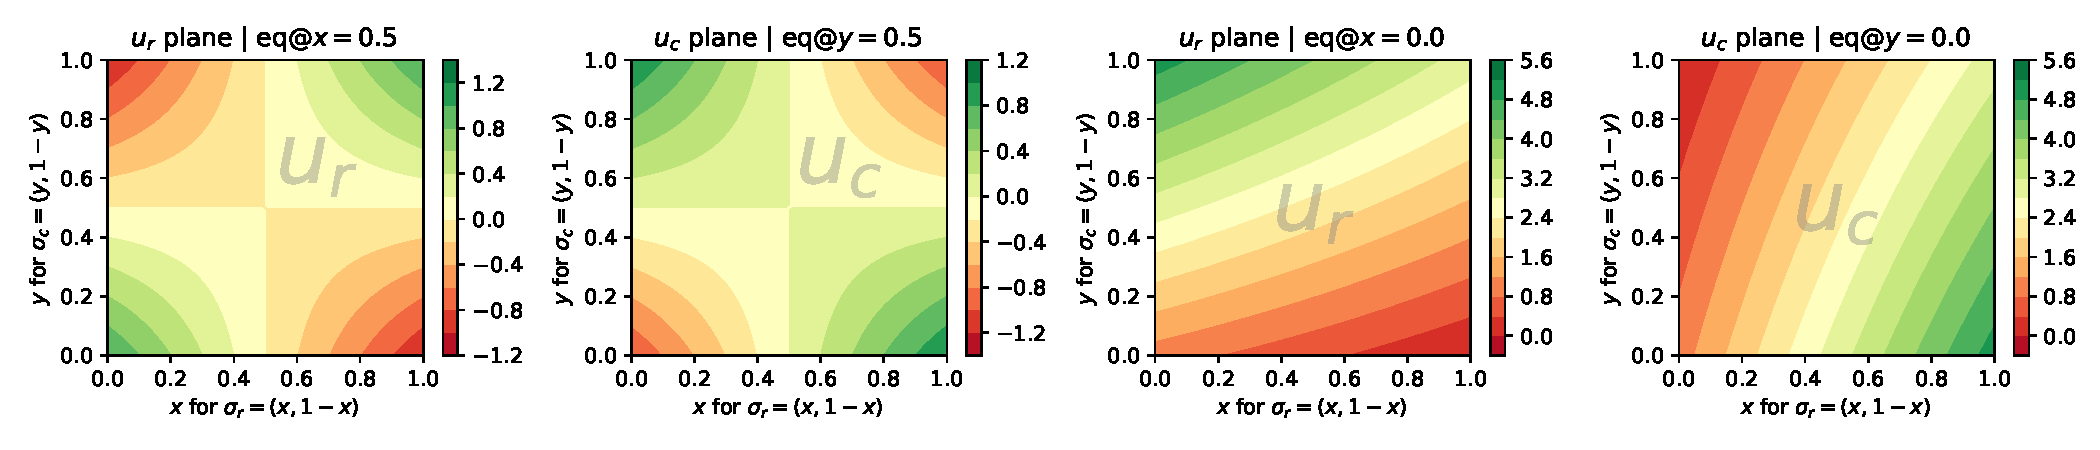
\includegraphics[width=1.0\textwidth, center]{./img/f1.pdf}
    \end{figure}
    \endgroup
    Here we see a filled contour plot of what the opponents are doing and the respective play off utility for a single turn of moves. The axis represents how players can form a strategy space but only control 1 axis; the row player controls $x$ and the column player controls $y$. For example, in the MP game (left pair) we can see that its best for players to play in the corners, however, the best utilities for players lie in opposite corners in the 2 utility planes; if a player was to try and play a corner (e.g $y=0$) the other player could exploit this ($x=1$). This is expected for zero-sum games because for one player to win in this type of game the other must lose. 

    The equilibria here can be seen to be $x=.5, \, y=.5$, as \mintinline{python}{nashpy} calculated, by observing the utility plane and asking, for both players, 'if I move can I score better?'. The answer is no. Consider moving $y$ to $0$, then $x$ could also move to $0$ and get an expected utility of $1$ leaving $u_c=-1$.
    
    The second game is The Prisoners Dilemma, a strongly dominated game. The Nash equilibria is less clear but by analysing the 2 utility matrices, and asking the question again, we can see that $x=0$, $y=0$ does make sense. The second strategy for both matrices is strongly dominant, i.e. playing anything other than $x=0$ and $y=0$ is irrational. 
   
    The process of asking 'if I set my variable differently can I score better?' in turn for each player will eventually end up with finding an equilibria. What were actually doing here is support enumeration, checking if positions across 2 positions are best responses to each other, this is more clear when we add more equilibria points to the examples. Below are made up games that have multiple equilibria points (the best responses are underlined): 
    \begingroup\makeatletter\def\f@size{8}\check@mathfonts
        $$ \text{LEFT:  }
            A=\begin{pmatrix}\underline1 & 0 \\ 0 & \underline1\end{pmatrix}\quad
            B=\begin{pmatrix}\underline1 & 0 \\ \underline0 & \underline0\end{pmatrix}\qquad\vert\qquad
        \text{RIGHT: }
            A=\begin{pmatrix}\underline2 & 0 \\ 0 & \underline3\end{pmatrix}\quad
            B=\begin{pmatrix}\underline3 & 0 \\ 0 & \underline2\end{pmatrix}$$
    \endgroup
    \begin{figure}[ht]
        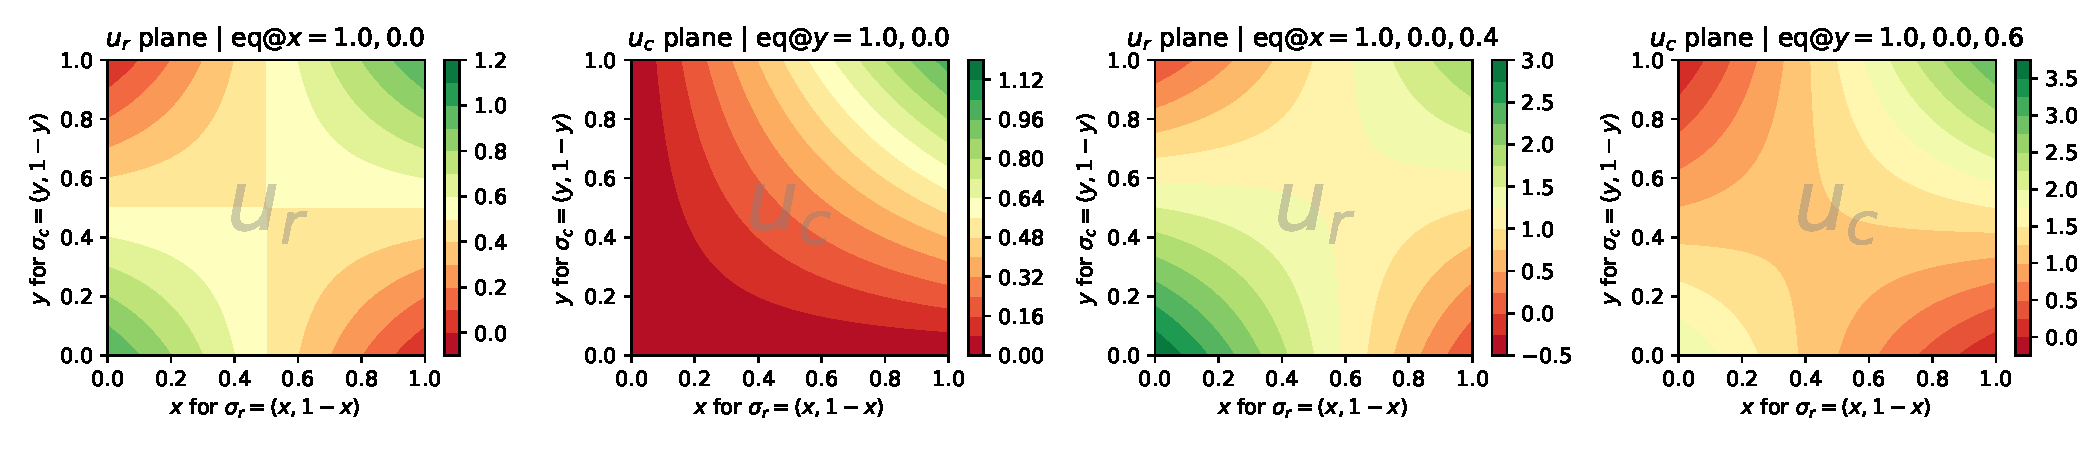
\includegraphics[width=1.0\textwidth, center]{./img/f2.pdf}
    \end{figure}

    Lets think of the support enumeration algorithm, the first step is to identify best responses support size $1$. The above matrices have matching best responses when the position in both $A$ and $B$ are underlined and thus an equilibria. In the left game there are 2, at $\sigma_r=(1,0),\, \sigma_c=(1,0)$ and $\sigma_r=(0,1),\, \sigma_c=(0,1)$. This also holds for the right game too. Looking at the plane this is clear because both players will benefit from these positions and have no reason to move.

    What is more difficult to see is the equilibria $\sigma_r=(0.4,0.6),\, \sigma_c=(0.6,0.4)$ of the right game. In the support enumeration algorithm this corresponds to the solving of best response mixed strategies of support size 2:
    \begingroup\makeatletter\def\f@size{8}\check@mathfonts
     $$ 
        \sum_{i\in I} \sigma_{r_i} B_{ij} = v \, \forall j \in J \quad \text{or} \quad
        \begin{pmatrix} \sigma_{r_1} & \sigma_{r_2} \end{pmatrix}
        \begin{pmatrix} 3 & 0 \\ 0 & 2 \end{pmatrix}
        = 
        \begin{pmatrix} v & v \end{pmatrix}
        \Rightarrow
        3 \sigma_{r_1} = 2 \sigma_{r_2}
        \Rightarrow
        3 x = 2(1-x) 
        \Rightarrow
        x=2/5 = 0.4
        $$
    and 
    $$ 
        \sum_{j\in J} A _{ij} \sigma_{c_j}^T = u \, \forall i \in I \quad \text{or} \quad
        \begin{pmatrix} 2 & 0 \\ 0 & 3 \end{pmatrix}
        \begin{pmatrix} \sigma_{c_1} \\ \sigma_{c_2} \end{pmatrix}
        = 
        \begin{pmatrix} u \\ u \end{pmatrix}
        \Rightarrow
        2 \sigma_{c_1} = 3 \sigma_{c_2}  
        \Rightarrow
        2 y = 3(1-y) 
        \Rightarrow
        y=3/5 = 0.6$$
    \endgroup
    These equations represent providing an opponent with an indifferent choice of utility for their strategy. If, for both players, the calculated mixed strategy is the best response to their opponents calculated mixed strategy then a nash equilibria has been found. This result can be visually understood by identifying that the a players choice of mixed strategy sits on the inflection point of the utility plane of the their opponent. This means that each player must actively decide to play their opponents inflection point or be taken advantage of; i.e. they provide an indifferent choice of utility to their opponent while also being provided an indifferent  utility choice.

    The relationship between pairs of visual utility planes and the calculated best responses can easily describe an example. Imagine you, the row player, are busy at home with your new puppy and have $\sigma_r=($ignore$,$ pet$)$ while the puppy has $\sigma_c=($come to you$,$ run away$,$ play with a toy$)$. This leads pay off matrices:
    \begingroup\makeatletter\def\f@size{8}\check@mathfonts
    $$
    A = \begin{pmatrix} 2 & 2 & -6 \\ \underline6 & \underline6 & \underline3 \\ \end{pmatrix}
    \qquad \vert \qquad
    B = \begin{pmatrix} \underline4 & 2 & \underline4 \\ \underline6 & -1 & \underline6 \\ \end{pmatrix}
    $$
    \endgroup
    \begin{figure}[!b]
        \centering
        \begin{minipage}{0.48\textwidth}
            \centering
            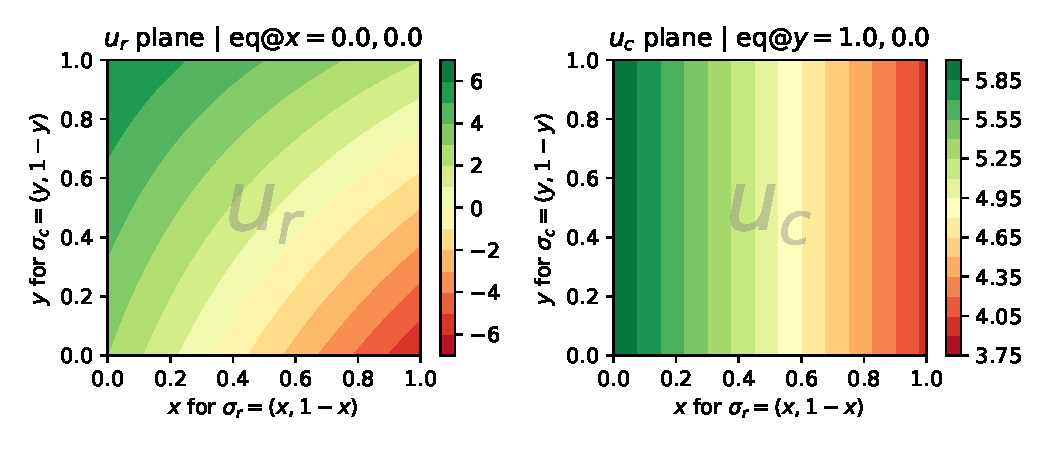
\includegraphics[width=1.0\textwidth, center]{./img/f3.pdf}
        \end{minipage}\hfill
        \begin{minipage}{0.48\textwidth}
            \inputminted[fontsize=\small]{python}{./code/nashpy-ex.py} 
        \end{minipage}
    \end{figure}
    Immediately it can be seen that this game reduces to a strongly dominant matrix $A$ (always pet the puppy) vs the non dominant $B$ (dogs love toys or cuddles). This leads to the outcome that the row player will always play his dominant strategy and the column player has no control over his own score. An interesting observation is that because of the strongly dominant nature of $A$ the row player can play any $\sigma_c=(y,0,1-y)\quad \forall y \in [0,1]$. This leads us to an interesting outcome; there are infinite nash equilibria: $x=0,\, y\in[0,1]$ the strategy $\sigma_r=(0,1)$ has any response by the column player as a best response, giving an example of a degenerate game.
    
        \newpage    
        APPENDIX
        \begin{figure}[ht]
            \inputminted[fontsize=\tiny]{python}{./code/plottingCode.py}
            \caption{Extended plotting code that was used to output figures.}
        \end{figure}
    
    \end{document}